\chapter{Kort}
\label{kort}

\begin{center}

\includegraphics[scale=0.8]{images/implementation/kort-icon_with_gloss}

{\large \textbf{\url{http://kort.herokuapp.com/}}}

\vspace{1cm}

\begin{figure}[H]
\subfigure{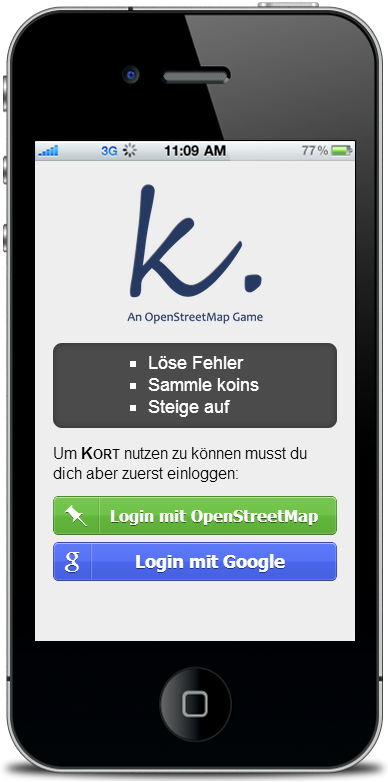
\includegraphics[width=0.3\textwidth]{images/screenshots/kort-screenshot-login}}
\hfill
\subfigure{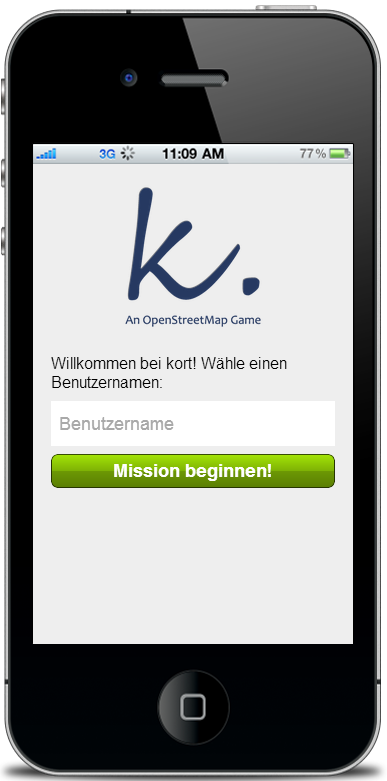
\includegraphics[width=0.3\textwidth]{images//screenshots/kort-screenshot-choose_username}}
\hfill
\subfigure{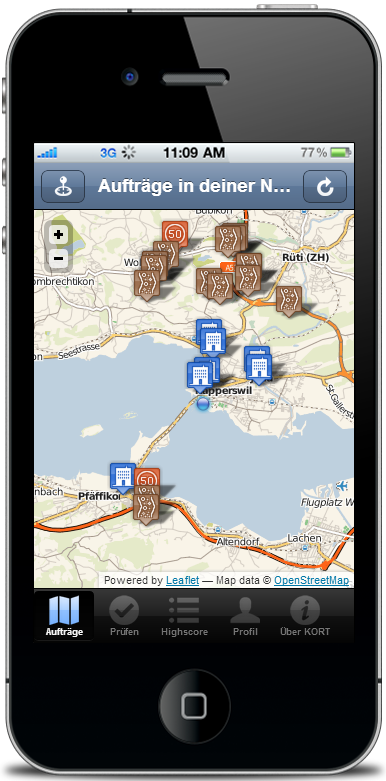
\includegraphics[width=0.3\textwidth]{images/screenshots/kort-screenshot-bugmap}}
\end{figure}
\end{center}

% Einführung
\section{Einführung}
\subsection{Idee}


% Ziel
\subsection{Ziel}


% Analyse
\section{Analyse}

\subsection{Paper-Prototype}
Vor der Implementation der Oberfläche wurde ein Paper-Prototype des GUI-Designs erstellt. Dieses wurde von verschiedenen Personen getestet. Der Prototype besteht aus drei verschiedenen Hauptmasken.

\subsubsection{Maske: Defekt melden}
Auf dieser Maske können Defekte gemeldet werden. Dazu lässt sich zuerst der Defekt-Typ wählen. Danach kann man auf der Karte den Standort des Defekts auswählen indem man die Defekt-Markierung darauf verschiebt. Abschliessend lässt sich die Meldung absenden.

\begin{figure}[H]
\subfigure[Defekt melden - Übersicht]{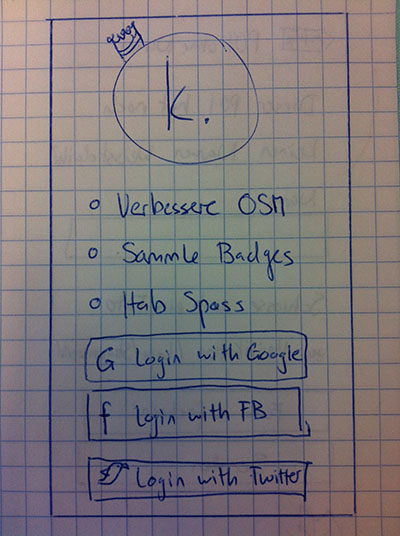
\includegraphics[width=0.43\textwidth]{images/paperprototype/kort-pp-startscreen}}
\hfill
\subfigure[Fehleranzeige beim Absenden ohne Defekttyp-Auswahl]{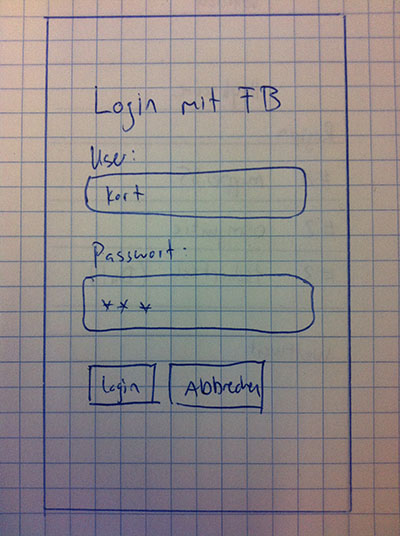
\includegraphics[width=0.43\textwidth]{images/paperprototype/kort-pp-login}}
\end{figure}